\documentclass[a4paper]{article}
\usepackage[english]{babel}
\usepackage[utf8x]{inputenc}
\usepackage[T1]{fontenc}
\usepackage{listings}
\usepackage[a4paper,top=2cm,bottom=2cm,left=2cm,right=2cm,marginparwidth=1.75cm]{geometry}
\usepackage{amsmath}
\usepackage{graphicx}
\usepackage[colorinlistoftodos]{todonotes}
\usepackage[colorlinks=true, allcolors=blue]{hyperref}
\setlength\parindent{0pt} % indent

\usepackage{mathtools}

% my commands:
\newcommand{\n}{\newline}
\newcommand{\tab}{\hspace{1cm}}
\newcommand{\dx}{\text{d}x}
\newcommand{\dy}{\text{d}y}
\newcommand{\dt}{\text{d}t}
\newcommand{\sgn}{\text{sgn}}

\begin{document}
\vspace{-4cm}
{\fontfamily{pbk}\fontsize{12}{15}\selectfont \hspace{-0.5cm}\text{4. domácí úkol | Vilém Zouhar}}

\section{}
\begin{align*}
	& \text{Původní funkce je definovaná na: } \mathbf{R} \backslash \bigcup_{k\in \mathbf{Z}} \{ k\pi \} \\
	& \int \frac{1}{\sin^2(x)+ \tan^2(x)} \dx = \bigg[\textit{sub. } t = \tan(x), 1\cdot dx = \frac{1}{1+t^2} dt, \cos^2 x = \frac{1}{1+t^2}, \sin^2 x = 1-\frac{1}{t^2+1}=\frac{t^2}{t^2+1} \bigg] = \\
	& \int \frac{1}{\frac{t^2}{t^2+1} + t^2 } \cdot \frac{1}{t^2+1} \dt = \int \frac{1+t^2}{(t^2 + t^2 + t^4)\cdot (1+t^2)} \dt = \int \frac{1}{t^2(2+t^2)} \dt = \\
	& \hspace{1cm} \bigg[ \frac{1}{2t^2 + t^4}  = \frac{A}{t} + \frac{B}{t^2} + \frac{Ct+D}{t^2+2} \Rightarrow (A, B, C, D) = (0, 1/2, 0, -1/2) \bigg]\\
	& = \frac{1}{2} \int \frac{1}{t^2} \dt - \frac{1}{2} \int \frac{1}{2+t^2} \dt = \\
	& \hspace{1cm} \int \frac{1}{t^2} \dt = \frac{-1}{t} + c_1 \\
	& \hspace{1cm} \int \frac{1}{2+t^2} = \frac{1}{\sqrt{2}} \int \frac{\frac{1}{\sqrt{2}}}{1+\big(\frac{t}{\sqrt{2}}\big)^2} \dt = \bigg[\textit{sub. } y = \frac{t}{\sqrt{2}}, y' = \frac{1}{\sqrt{2}} \bigg] = \frac{1}{\sqrt{2}} \int \frac{1}{1+ y^2} = \frac{1}{\sqrt{2}} \arctan(y) + c_2 \\
	& \hspace{14cm} = \frac{1}{\sqrt{2}} \arctan(\frac{t}{\sqrt{2}}) + c_2 \\
	& = \frac{-1}{2t} - \frac{1}{2\sqrt{2}} \arctan\Big(\frac{t}{\sqrt{2}}\Big) + c = \frac{-1}{2\tan(x)} - \frac{1}{2\sqrt{2}} \arctan\Big(\frac{\tan(x)}{\sqrt{2}}\Big) + c \\
	& \text{Kvůli prvnímu zlomku je třeba vyloučit $k\pi$, navíc je limita arctan v $\pm \infty$ různá, proto i $k\pi + \pi/2$: } \\
	& \text{primitivní funkce na intervalech: } \mathbf{R} \backslash \bigcup_{k\in \mathbf{Z}} \{ k\pi/2 \}
\end{align*}

\section{}
\begin{align*}
	& \text{Původní funkce je definovaná na: } \mathbf{R} \\
	& \int |\sin(x) + \cos(x)| \dt = [\text{dle integrování funkce v absolutní hodnotě}] = (\sin(x) - \cos(x))\cdot \sgn (\sin(x) + \cos(x)) + c \\
	& \text{Tato funkce je však nespojitá v bodech $k\pi - \pi/4$ (sgn převrací znaménko)} \\
	& \text{}\hspace{2cm}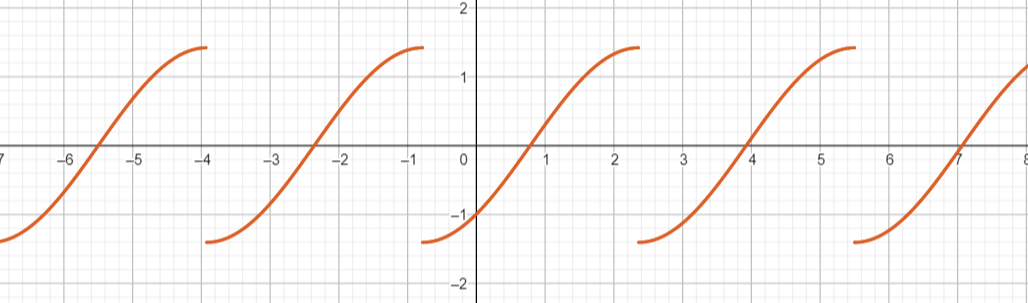
\includegraphics[height=4cm]{trigo_fun} \\
	& \text{Označme části funkce: } F_i = (\sin(x) - \cos(x))\cdot \sgn (\sin(x) + \cos(x)) + c + i\cdot M \text{ na intervalu } (i\cdot \pi + 3\pi/4, i\cdot \pi + 3\pi/4) \\
	& \text{Chybějící body v $i\cdot\pi - \pi/4$ dodefinujeme pro spojitost (kvůli nulovému sgn) jako $i \cdot M+q+c$ }\hspace{0.2cm} q, c, M \in \mathbf{R} \\
	& F_0 = (\sin(x) - \cos(x))\cdot \sgn (\sin(x) + \cos(x)) + c \\
	& F_1 = (\sin(x) - \cos(x))\cdot \sgn (\sin(x) + \cos(x)) + c + M, \dots \\
	& \text{Je třeba nyní najít správné konstanty $M, q$, které funkci poslepují do spojité. } \\
	& \text{Stačí přičíst rozdíl v bodech  $i\cdot \pi - \pi/3$ a $i\cdot \pi + 3\pi/4$, což je vždy $2\sqrt{2} = M$, pak $q = \sqrt{2}$}. \\
	& \text{Předpis pro funkci je tedy: } F(x) = 
		\begin{cases*}
		(\sin(x) - \cos(x))\cdot \sgn  (\sin(x) + \cos(x)) + c + i\cdot 2 \sqrt{2} & $x \in (i\cdot \pi - \pi/4, i\cdot \pi + 3\pi/4)$ \\
		i \cdot 2\sqrt{2}+\sqrt{2} + c & $x = i\cdot \pi + 3\pi/4$
		\end{cases*} \\
	& \hspace{15cm} i \in \mathbf{Z}, c \in \mathbf{R}, x \in \mathbf{R}
\end{align*}

\section{}
\begin{align*}
	& \text{Původní funkce je definovaná na: } \mathbf{R} \backslash  \{ 1 \} \\
	& \int \frac{8+6x-2x^2}{x^4-4x+3} \dx = \int \frac{8+6x-2x^2}{(x-1)^2(x^2+2x+3)} = \dx \\
	& \hspace{1cm} \bigg[ \frac{8+6x-2x^2}{(x-1)^2(x^2+2x+3)}  = \frac{A}{x-1} + \frac{B}{(x-1)^2} + \frac{Cx+D}{x^2+2x+3} \Rightarrow (A, B, C, D) = (-1, 2, 1, -1) \textit{ (za pomocí eliminace)}\bigg] \\
	&  = - \int \frac{1}{x-1} \dx + 2 \int \frac{1}{(x-1)^2} \dx + \int \frac{x-1}{x^2+2x+3} \dx = \\
	& = - \int \frac{1}{x-1} \dx + 2 \int \frac{1}{(x-1)^2} \dx + \frac{1}{2} \int \frac{2x+2}{x^2+2x+3}-2 \int \frac{1}{x^2+2x+3} = \dx \\	
	& \hspace{1cm} \int \frac{1}{x-1} \dx = \ln|x-1|+c_1 \\
	& \hspace{1cm} \int \frac{1}{(x-1)^2} \dx = -(x-1)^{-1}+c_2 \\
	& \hspace{1cm} \int \frac{2x+2}{x^2+2x+3} \dx =[\textit{sub. } y = x^2+2x+3, y' = 2x+2] = \int \frac{1}{y} \dy = \ln|y| + c_3 = \ln|x^2+2x+3| + c_3 \\  
	& \hspace{1cm} \int \frac{1}{x^2+2x+3} = \frac{1}{\sqrt{2}} \int \frac{\frac{1}{\sqrt{2}}}{(\frac{x+1}{\sqrt{2}})^2+1} \dx =[\textit{sub. } y = (x+1)/\sqrt{2}, y' = 1/\sqrt{2}] = \\
	& \hspace{8cm} \frac{1}{\sqrt{2}} \int \frac{1}{y^2+1} \dy = \frac{1}{\sqrt{2}} \arctan(y) + c_4 = \frac{1}{\sqrt{2}} \arctan((x-1)/\sqrt{2}) + c_4 \\
	& = - \ln|x-1| -2(x-1)^{-1}+ \frac{1}{2} \ln|x^2+2x+3|-\sqrt{2} \arctan((x-1)/\sqrt{2}) + c \\
	& \text{Kvůli zlomku a logaritmu je třeba vyloučit $x = 1$, proto je primitivní funkce definovaná na: } (-\infty, 1)\ a\ (1, \infty)\\
\end{align*}
\end{document}
